
\documentclass{article}

% Required packages
\usepackage{amssymb}
\usepackage{amsmath}
\usepackage{graphicx}
\usepackage{geometry}
\usepackage{tikz}
\usepackage{array}
\usepackage{booktabs}
\usepackage{enumitem}
\usepackage{listings}
\usepackage{xcolor}
\usepackage{fancyhdr}
\usepackage{float}
\usepackage{subcaption}

% Set page geometry
\geometry{a4paper, margin=1in}

% Configure listings for Python
\lstset{
  language=Python,
  basicstyle=\ttfamily\footnotesize,
  numbers=left,
  numberstyle=\tiny\color{gray},
  frame=single,
  breaklines=true,
  breakatwhitespace=true,
  captionpos=b,
  tabsize=4,
  showspaces=false,
  showstringspaces=false,
  showtabs=false,
  commentstyle=\color{gray}\textit,
  keywordstyle=\color{blue}\bfseries,
  stringstyle=\color{red}
}

\begin{document}

\pagestyle{fancy}
\chead{DSC 255: Machine Learning Fundamentals (Spring 2025)}
\lhead{Homework 7}
\rhead{Randall Rogers}

\subsection*{Solution 1}
\noindent\rule{\textwidth}{0.4pt}\\

% -----------------------------------------------------------------
\subsubsection*{Step 1}
\parbox{\textwidth}{
The general form for a linear predictor is the following:

$$f(x) = w^{T}x + b$$\\

We are given three linear functions for each class:

$$\text{Class 1: } w_1=(1,1), b_1 = 0 \rightarrow f_{1}(x) = x_{1}\cdot(w^1_1)+x_{2}\cdot(w^1_2)+b_1 = x_{1}\cdot(1)+x_{2}\cdot(1)+0 = x_{1} + x_{2} $$\\
$$\text{Class 2: } w_2=(1,0), b_2 = 1 \rightarrow f_{2}(x) = x_{1}\cdot(w^2_1)+x_{2}\cdot(w^2_2)+b_2 = x_{1}\cdot(1)+x_{2}\cdot(0)+1 = x_{1} + 1 $$\\
$$\text{Class 3: } w_3=(0,1), b_3 = -1 \rightarrow f_{3}(x) = x_{1}\cdot(w^3_1)+x_{2}\cdot(w^3_2)+b_3 = x_{2}\cdot(0)+x_{1}\cdot(1)-1 = x_{2} - 1$$\\

Hence, for each class, we have the following:

$$
\begin{aligned}
f_{1}(x) &= x_{1}+x_{2},\\
f_{2}(x) &= x_{1}+1,\\
f_{3}(x) &= x_{2}-1.
\end{aligned}
$$
}
% -----------------------------------------------------------------
\subsubsection*{Step 2}
\parbox{\textwidth}{
Compare $f_{1}$, $f_{2}$, and $f_{3}$ at the intersection points of the decison boundaries:

\begin{center}
$$
\begin{aligned}
\text{(1 vs 2)} &: \; f_{1}=f_{2} \;\rightarrow\; x_{1}+x_{2} = x_1 + 1 \;\rightarrow\; x_{2} = 1 \;\rightarrow\; (0,1)\\
\text{(1 vs 3)} &: \; f_{1}=f_{2} \;\rightarrow\; x_{1}+x_{2} = x_2 - 1 \;\rightarrow\; x_{1} = -1 \;\rightarrow\; (-1,0) \\
\text{(2 vs 3)} &: \; f_{2}=f_{3} \;\rightarrow\; x_{1}+1 = x_{2}-1 \;\rightarrow\; x_{2} = x_{1}+2 \;\rightarrow\; (0,2) \text{ and }  (-2,0)\\
\end{aligned}
$$
\end{center}

Hence, we have the following decision boundaries:
\begin{center}
$$
\begin{aligned}
\text{Decision Boundary between Class 1 and Class 2: }& \quad x_{2}=1 \\
\text{Decision Boundary between Class 1 and Class 3: }& \quad x_{1}=-1 \\
\text{Decision Boundary between Class 2 and Class 3: }& \quad x_{2}=x_{1}+2 
\end{aligned}
$$
\end{center}
}

\subsubsection*{Step 3}
\parbox{\textwidth}{
Note: \,$x_{2}=1$, \,$x_{1}=-1$, and \,$x_{2}=x_{1}+2$ all pass
through the common point $(-1,1)$,and slice the plane into 6 wedges.\\

Now, select six test points for each wedge, and evaluate $f_1$, $f_2$, and $f_3$ to determine the classification.\\

$$
\begin{array}{c|c|c|c|c|c}
\text{Wedge label} & \text{Test point} & f_{1}(x) & f_{2}(x) & f_{3}(x) & \text{Classification}\\ \hline
A & ( 1, 4)  &  5 &  2 &  3 & \text{Class 1}\\ %  x_{1}>-1, x_{2}>1,  below red
B & ( 1, 2)  &  3 &  2 &  1 & \text{Class 1} \\ %  x_{1}>-1, 1<x_{2}<x_{1}+2
C & ( 1, -1) &  0 &  2 & -2 & \text{Class 2}\\ %  x_{1}>-1, x_{2}<1
D & (-2,-1)  & -4 & -1 & -3 & \text{Class 2}\\ %  x_{1}<-1, x_{2}<1, below red
E & (-3, 0)  & -3 & -2 & -1 & \text{Class 3}\\ % x_{1}<-1, x_{2}<1,
F & (-3, 3)  &  0 & -2 &  2 & \text{Class 3}\\ %  x_{1}<-1, x_{2}>1
\end{array}
$$

}

\subsubsection*{Step 4}
\parbox{\textwidth}{
Visualize points and classify each wedge.
}
\begin{figure}[h]
\centering
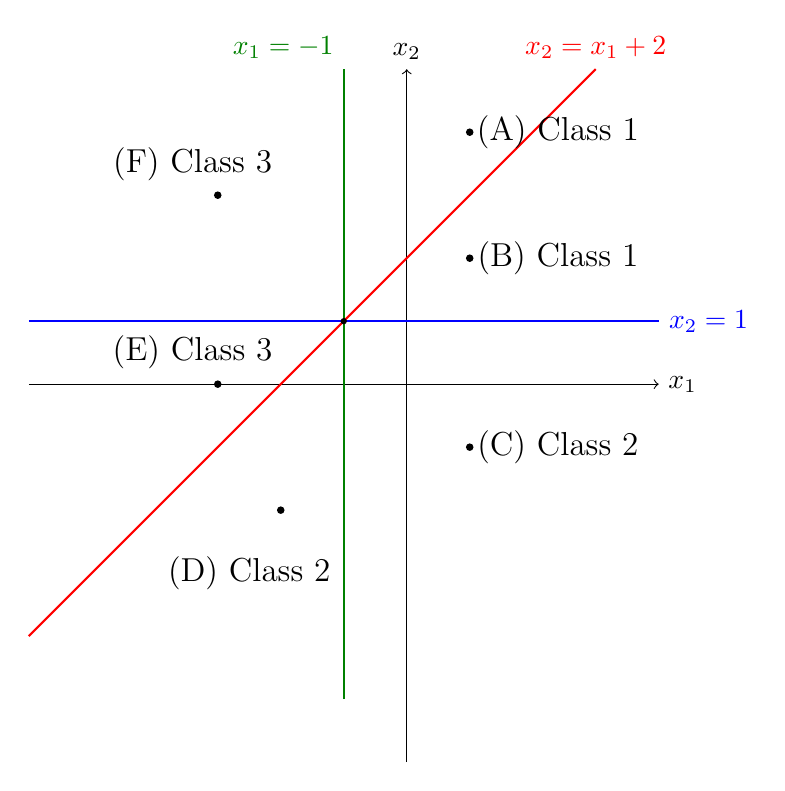
\begin{tikzpicture}[scale=0.8]

% Axes
\draw[->] (-6,0) -- (4,0) node[right] {$x_{1}$};
\draw[->] (0,-6) -- (0,5) node[above] {$x_{2}$};

% Decision boundaries
\draw[blue,thick] (-6,1) -- (4,1)   node[right] {$x_{2}=1$};          % 1 vs 2
\draw[green!50!black,thick] (-1,-5) -- (-1,5) node[above left] {$x_{1}=-1$}; % 1 vs 3
\draw[red,thick] (-6,-4) -- (3,5)   node[above] {$x_{2}=x_{1}+2$};     % 2 vs 3

% Intersection point
\fill (-1,1) circle (0.05);

% Class labels in each wedge
\node at ( 2.4, 4) {\large (A) Class 1};
\node at ( 2.4, 2) {\large (B) Class 1};

\node at ( 2.4,-1) {\large (C) Class 2};
\node at (-2.5,-3) {\large (D) Class 2};

\node at (-3.4, 0.5) {\large (E) Class 3};
\node at (-3.4, 3.5) {\large (F) Class 3};

% (Optional) test points used to verify labels
\fill ( 1,4)   circle (0.06);
\fill ( 1,2) circle (0.06);
\fill ( 1,-1)   circle (0.06);
\fill (-2,-2)  circle (0.06);
\fill (-3,0) circle (0.06);
\fill (-3,3)   circle (0.06);

\end{tikzpicture}
\caption{All six wedges produced by the three pairwise boundaries, with the winning class shown in each.}
\end{figure}

% -----------------------------------------------------------------
\subsubsection*{\normalfont}
{
$\therefore$ the decision boundaries and the regions that belong to each class can be seen in \textit{Figure 1}.
}\\
\noindent\rule{\textwidth}{0.4pt}\\

\newpage

\subsection*{Solution 2}
\noindent\rule{\textwidth}{0.4pt}\\

% -----------------------------------------------------------------
\subsubsection*{Step 1}
\parbox{\textwidth}{
In order to determine which option will best satisfy the statistical learning framework, we will evaluate each option.
\begin{itemize}
    \item Option A: A web search on \textit{American plants} will yeild subset of plant images outside of California.
    \item Option B: Plant photos from a similar region to that of California, will yeild similar flora but not identiencal to Californian flora.
    \item Option C: Plant photos from the favorite Californian city will yeild photos of plants will have a higher bias towards urban Californian flora.
\end{itemize} 
}
\subsubsection*{\normalfont}{$\therefore$ Option B will best satisfy the statistical learning framework, since it will introduce the least amount of bias towards Californian plant identification.}\\

\noindent\rule{\textwidth}{0.4pt}\\

\newpage
\subsection*{Solution 3}
\noindent\rule{\textwidth}{0.4pt}\\

\subsubsection*{Step 1}
\parbox{\textwidth}{
We will explore a few potential reasons why the SVM classifier performs well despite the large number of features.
\begin{itemize}
\item If the classes the SVM is predicting are sufficently different, the SVM will be able to find a good decision boundary that separates the data.
      As a consquence of the difference between the classes, the SVM will have a large margin. This means that the SVM can find a good decision boundary even with a large number of features and minimal training points.

\item The generalizaton error can be  expressed as:
      \[
        \text{generalisation error} \;\approx\; 
        \sqrt{\dfrac{R^{2}/\gamma^{2}}{n}}
      \]
      So we can see that as the margin grows largers, the generalization error decreases. This means that the SVM can find a good decision boundary even with a large number of features and minimal training points.

\end{itemize}
}

\subsubsection*{\normalfont}{$\therefore$ a wide margin for the SVM is a key reason the 1000 traing points are sufficent reguardless of the one million features in the data.}

\noindent\rule{\textwidth}{0.4pt}\\

\newpage

\subsection*{Solution 4 (a)}
\noindent\rule{\textwidth}{0.4pt}\\

\subsubsection*{\normalfont}{The class priors changed: fewer \textit{sports} articles, more \textit{politics} Within each topic (class), the way the text is written is assumed unchanged, so only the frequency of each label moves.
}
\subsubsection*{\normalfont}{$\therefore$ this would be an example of a label shift}

\noindent\rule{\textwidth}{0.4pt}\\

\subsection*{Solution 4 (b)}
\noindent\rule{\textwidth}{0.4pt}\\

\subsubsection*{\normalfont}{The vocabulary has drifted: new proper nouns appear and old ones vanish. This alters the distribution of the features within each topic, while the overall mix of topics (sports, politics, business,etc.) stays the same.}

\subsubsection*{\normalfont}{$\therefore$ this is an example of a covariate shift}

\noindent\rule{\textwidth}{0.4pt}\\



\end{document}


